\chapter{Phép đo, ma trận mật độ và entropy}

Thí nghiệm hai khe chứa đựng vấn đề đo lường ở dạng đơn giản nhất vẫn hữu ích. Khi hai khả năng còn giữ được tính kết hợp, các biên độ giao thoa với nhau. Khi một hệ khác ghi nhận khả năng nào đã xảy ra, hạt và thiết bị ghi nhận trở nên rối với nhau, làm thay đổi sự giao thoa. Trước khi giới thiệu phép lấy vết, ma trận mật độ và entropy---, ta sẽ mô tả chính xác cơ chế ấy; đó là những khái niệm cần thiết để định lượng sự rối.

\section{Dựng lại thí nghiệm hai khe}

Xét một mô hình rời rạc, trong đó nguồn đặt tại vị trí \(0\), hai khe ở \(A\) và \(B\), còn các vị trí có thể đến trên màn được biểu diễn bằng các trạng thái trực chuẩn \(\{|m\rangle\}\). Hạt có thể là electron, photon hoặc bất kỳ đối tượng lượng tử nào khác. Ta gọi nó là electron và bỏ qua spin riêng của nó, để vị trí là bậc tự do duy nhất đang xét. Phần còn lại của rào chắn được đóng kín: electron đến bất kỳ vị trí nào ngoài \(A\) hoặc \(B\) đều bị phản xạ.

Nguyên lý nền tảng ở đây là tính tuyến tính. Nếu hai trạng thái tiến hóa theo
\begin{equation}
|A\rangle\longrightarrow |A'\rangle,
\qquad
|B\rangle\longrightarrow |B'\rangle,
\end{equation}
thì mọi chồng chập cũng tiến hóa với đúng các hệ số ấy:
\begin{equation}
\alpha|A\rangle+\beta|B\rangle
\longrightarrow
\alpha|A'\rangle+\beta|B'\rangle.
\end{equation}

Trong cách bố trí đối xứng, nguồn cấp cho hai khe các biên độ bằng nhau. Lược bỏ hệ số chuẩn hóa chung như trên bảng,
\begin{equation}
|0\rangle\longrightarrow |A\rangle+|B\rangle.
\end{equation}
Trạng thái đã chuẩn hóa sẽ là \((|A\rangle+|B\rangle)/\sqrt{2}\); hệ số bị lược bỏ không ảnh hưởng đến lập luận về giao thoa.

Giờ hãy xét riêng từng đường đi. Quá trình truyền từ các khe đến màn có dạng
\begin{align}
|A\rangle &\longrightarrow \sum_m \psi_m|m\rangle, \\
|B\rangle &\longrightarrow \sum_m \phi_m|m\rangle.
\end{align}
Số phức \(\psi_m\) là biên độ để hạt đến vị trí \(m\) trên màn khi xuất phát từ \(A\), còn \(\phi_m\) là biên độ tương ứng khi xuất phát từ \(B\).

\begin{figure}[htbp]
\centering
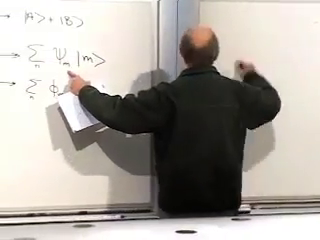
\includegraphics[width=0.68\textwidth]{lecture_07_figure_02.png}
\caption{Các khai triển riêng cho đường đi \(A\) và \(B\) trong cơ sở trên màn.}
\lectureframe{00:05:39}
\end{figure}

Nếu đóng \(B\), xác suất tại \(m\) là
\begin{equation}
P_A(m)=|\psi_m|^2.
\end{equation}
Nếu đóng \(A\),
\begin{equation}
P_B(m)=|\phi_m|^2.
\end{equation}
Theo xác suất cổ điển, ta có thể nghĩ rằng khi mở cả hai khe thì cộng hai kết quả này. Nhưng cơ học lượng tử cộng các biên độ trước:
\begin{equation}
|A\rangle+|B\rangle
\longrightarrow
\sum_m(\psi_m+\phi_m)|m\rangle.
\end{equation}
Tại một vị trí cố định trên màn,
\begin{align}
P(m)
&=|\psi_m+\phi_m|^2 \\
&=|\psi_m|^2+|\phi_m|^2
  +\psi_m^*\phi_m+\phi_m^*\psi_m.
\end{align}

\begin{figure}[htbp]
\centering
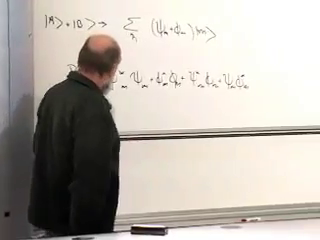
\includegraphics[width=0.70\textwidth]{lecture_07_figure_03.png}
\caption{Xác suất tại màn gồm bốn số hạng. Hai số hạng cuối là các số hạng giao thoa.}
\lectureframe{00:09:21}
\end{figure}

Tại một điểm đối xứng, \(\psi_m=\phi_m\), nên hai khả năng tăng cường lẫn nhau. Tại một điểm mà pha của chúng lệch nhau \(\pi\), \(\psi_m=-\phi_m\), xác suất triệt tiêu. Đi riêng theo đường nào cũng có thể đến điểm đó, vậy mà mở cả hai đường lại có thể khiến electron không đến được đó. Giờ đây không thể tránh câu hỏi: điều gì thay đổi khi có thứ gì đó ghi lại khe nào đã được sử dụng?

\section{Thiết bị dò trở nên rối với hệ}

Ta đưa vào một hệ phụ hai trạng thái, với các trạng thái \(|u\rangle\) và \(|d\rangle\). Trong mô hình này, đó không phải spin của electron mà là một thiết bị bên ngoài tối giản. Ban đầu, thiết bị dò chưa được kích hoạt:
\begin{equation}
|0,d\rangle.
\end{equation}
Bố trí tương tác sao cho khi đi qua \(A\), thiết bị dò lật trạng thái; còn khi đi qua \(B\), trạng thái của nó không đổi:
\begin{equation}
|0,d\rangle
\longrightarrow
|A,u\rangle+|B,d\rangle.
\end{equation}
Sau khi electron rời khỏi các khe, nó không còn tương tác với spin phụ nữa. Vì vậy, hai nhánh lan truyền theo
\begin{align}
|A,u\rangle &\longrightarrow \sum_m\psi_m|m,u\rangle, \\
|B,d\rangle &\longrightarrow \sum_m\phi_m|m,d\rangle,
\end{align}
và trạng thái cuối cùng là
\begin{equation}
|\Psi\rangle
=\sum_m\left(\psi_m|m,u\rangle+\phi_m|m,d\rangle\right).
\end{equation}
Đường đi và thông tin ghi nhận bởi thiết bị dò giờ đã rối với nhau. Đọc trạng thái thiết bị dò sẽ cho biết electron đã đi qua khe nào.

\begin{classroomqa}
\lecturetimestamp{00:13:24}
\audiencequestion{Gói sóng đã sụp đổ ngay khi spin lật trạng thái chưa?}
\lecturerresponse{Nếu chỉ xét electron, ta có thể dùng ngôn ngữ sụp đổ: các khả năng đường đi không còn giao thoa với nhau. Tuy nhiên, đối với toàn bộ hệ electron--thiết bị dò, không nhánh nào bị loại bỏ. Trạng thái vẫn là \(|A,u\rangle+|B,d\rangle\). Khi tính cả thiết bị, phát biểu \emph{electron đã sụp đổ} được thay bằng phát biểu chính xác rằng sự rối giữa hệ--thiết bị đã hình thành.}
\end{classroomqa}

Spin phụ chỉ là một con trỏ thuận tiện. Một thiết bị được kích hoạt hoặc chưa kích hoạt, một photon được phát ra hoặc không phát ra, hay bất kỳ cặp dấu ghi nhận phân biệt được nào khác đều có thể đảm nhiệm vai trò ấy.

\begin{classroomqa}
\lecturetimestamp{00:15:17}
\audiencequestion{Bản thân việc đi qua tấm kim loại có phải lúc nào cũng để lại dấu vết đường đi không?}
\lecturerresponse{Không nhất thiết. Điều quan trọng là tương tác có khiến tấm ở những trạng thái cuối cùng phân biệt được hay không. Nếu tấm có một khe năng lượng kích thích và electron không đủ năng lượng để kích thích nó thì có thể không để lại dấu vết nội tại lâu bền nào. Chỉ tương tác thôi là chưa đủ; hai khả năng phải tương quan với những dấu ghi nhận phân biệt được.}
\end{classroomqa}

\begin{classroomqa}
\lecturetimestamp{00:16:29}
\audiencequestion{Liệu độ giật lùi của tấm có thể cho biết electron đi qua khe trên hay khe dưới không?}
\lecturerresponse{Chỉ khi các cú giật lùi theo hai hướng động lượng ngược nhau tạo ra những trạng thái của tấm phân biệt được đủ rõ. Một tấm được định xứ tốt vốn đã có hàm sóng động lượng rộng. Những dịch chuyển nhỏ lên trên và xuống dưới có thể chồng lấp gần như hoàn toàn, nên các trạng thái giật lùi không trực giao và không cung cấp được dấu ghi nhận đường đi rõ ràng. Đây là lúc nguyên lý bất định bảo vệ sự giao thoa.}
\end{classroomqa}

Có thể có dấu ghi nhận không đầy đủ. Nếu thiết bị dò chỉ bị tác động nhẹ, hai trạng thái ghi nhận cuối cùng không nhất thiết trực giao. Khi ấy, giao thoa bị suy giảm chứ không bị triệt tiêu. Để tính toán hình thức, trước hết ta xét trường hợp giới hạn của một phép đo hoàn chỉnh:
\begin{equation}
\langle u|d\rangle=0.
\end{equation}

\section{Tính xác suất bằng toán tử chiếu}

Giờ ta tính xác suất electron đến một vị trí cố định \(m\) trên màn, mà không hỏi kết quả đo của thiết bị dò. Trong không gian Hilbert kết hợp, tính chất \emph{electron ở vị trí \(m\)} xác định một không gian con hai chiều, được sinh bởi
\begin{equation}
|m,u\rangle,\qquad |m,d\rangle.
\end{equation}
Toán tử chiếu tương ứng là
\begin{equation}
\Pi_m
=|m,u\rangle\langle m,u|
 +|m,d\rangle\langle m,d|.
\end{equation}

\begin{figure}[htbp]
\centering
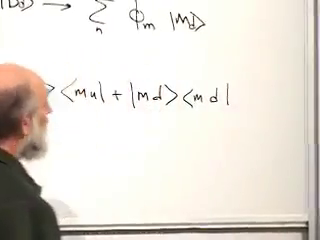
\includegraphics[width=0.66\textwidth]{lecture_07_figure_04.png}
\caption{Toán tử chiếu lên một vị trí cố định trên màn, lấy tổng theo hai trạng thái ghi nhận trực giao của thiết bị dò.}
\lectureframe{00:22:04}
\end{figure}

Tiên đề xác suất cho
\begin{equation}
P(m)=\langle\Psi|\Pi_m|\Psi\rangle.
\end{equation}
Viết các tổng ra,
\begin{align}
P(m)
&=
\sum_{n,n'}
\left(\psi_n^*\langle n,u|+\phi_n^*\langle n,d|\right)
\notag\\
&\quad\times\Pi_m
\notag\\
&\quad\times
\left(\psi_{n'}|n',u\rangle+\phi_{n'}|n',d\rangle\right).
\end{align}
Các tích vô hướng vị trí đòi hỏi \(n=m=n'\). Tiếp đó, các tích vô hướng của thiết bị dò quyết định những số hạng nào còn lại:
\begin{align}
\langle u|u\rangle&=1,
&
\langle d|d\rangle&=1,
&
\langle u|d\rangle&=\langle d|u\rangle=0.
\end{align}
Do đó,
\begin{equation}
P(m)=|\psi_m|^2+|\phi_m|^2.
\end{equation}

Các số hạng chéo không bị loại bỏ theo một quy ước áp đặt. Chúng triệt tiêu vì giờ đây các biên độ của hai đường đi nhân với những vectơ trực giao trong không gian trạng thái mở rộng. Muốn giao thoa, các khả năng không chỉ phải trùng nhau ở điểm cuối trên màn mà còn ở mọi bậc tự do mang thông tin ghi nhận.

\section{Thế nào được xem là một phép đo?}

Mô hình spin đơn giản đưa ra một quy tắc tổng quát: phép đo xảy ra khi tương tác thiết lập tương quan giữa các khả năng của hệ đang xét và những trạng thái phân biệt được của thiết bị đo. Các biến thể sau đây sẽ kiểm nghiệm quy tắc ấy.

\begin{classroomqa}
\lecturetimestamp{00:26:53}
\audiencequestion{Nếu đặt spin đối xứng và để nó lật trạng thái khi đi qua bất kỳ khe nào thì sao?}
\lecturerresponse{Khi ấy, cả hai nhánh đều mang cùng một dấu ghi nhận, \(|A,u\rangle+|B,u\rangle=(|A\rangle+|B\rangle)\otimes|u\rangle\). Trạng thái thiết bị dò tách ra khỏi trạng thái còn lại và không cung cấp thông tin về đường đi, nên hình giao thoa vẫn còn.}
\end{classroomqa}

\begin{figure}[htbp]
\centering
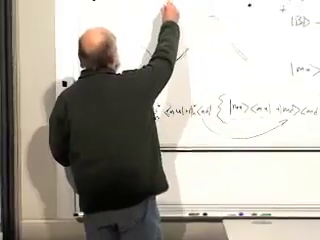
\includegraphics[width=0.68\textwidth]{lecture_07_figure_05.png}
\caption{Biến thể trên bảng, trong đó thiết bị dò đặt đối xứng và phản ứng như nhau với cả hai đường đi.}
\lectureframe{00:27:14}
\end{figure}

\begin{figure}[htbp]
\centering
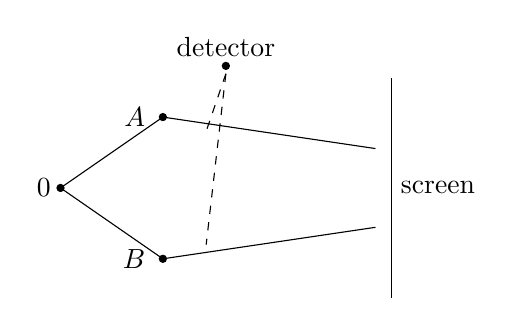
\begin{tikzpicture}[scale=1.0]
\fill (-2,0) circle (1.5pt);
\node[left] at (-2,0) {$0$};
\fill (-0.7,0.9) circle (1.5pt);
\node[left] at (-0.8,0.9) {$A$};
\fill (-0.7,-0.9) circle (1.5pt);
\node[left] at (-0.8,-0.9) {$B$};
\draw (-2,0) -- (-0.7,0.9);
\draw (-2,0) -- (-0.7,-0.9);
\draw (-0.7,0.9) -- (2.0,0.5);
\draw (-0.7,-0.9) -- (2.0,-0.5);
\draw (2.2,-1.4) -- (2.2,1.4);
\node[right] at (2.2,0) {screen};
\fill (0.1,1.55) circle (1.5pt);
\node[above] at (0.1,1.55) {detector};
\draw[dashed] (0.1,1.45) -- (-0.15,0.72);
\draw[dashed] (0.1,1.45) -- (-0.15,-0.72);
\end{tikzpicture}
\caption{Dựng lại bố trí thiết bị dò đối xứng: cả hai đường đi đều tạo ra cùng một trạng thái thiết bị dò.}
\end{figure}

\begin{classroomqa}
\lecturetimestamp{00:27:55}
\audiencequestion{Có cần ai đó thực sự đọc spin phụ thì giao thoa mới biến mất không?}
\lecturerresponse{Không. Electron đã tương quan đường đi của nó với spin. Ta có thể đặt lại thiết bị dò, lặp lại thí nghiệm từng electron một và chỉ kiểm tra phân bố các điểm chạm trên màn. Các vân giao thoa vẫn mất dù không ai đọc spin; điều quan trọng là dấu ghi nhận vật lý, chứ không phải con người có nhận biết nó hay không.}
\end{classroomqa}

\begin{classroomqa}
\lecturetimestamp{00:29:36}
\audiencequestion{Một tấm giật lùi đủ nhẹ có phá hủy giao thoa không?}
\lecturerresponse{Có, nếu cú giật lùi làm tấm chuyển sang các trạng thái động lượng trực giao ứng với hai đường đi. Nếu các gói sóng sau khi dịch chuyển vẫn chồng lấp, sự phá hủy chỉ là một phần. Khối lượng tự nó không phải tiêu chí; tiêu chí là khả năng phân biệt các trạng thái cuối cùng của tấm.}
\end{classroomqa}

Bức xạ là một thiết bị ghi nhận không hoàn hảo khác. Một hạt mang điện bị gia tốc có thể phát ra photon. Bức xạ phát ra gần \(A\) không nhất thiết ở cùng trạng thái với bức xạ phát ra gần \(B\), vì vậy trường điện từ có thể lưu giữ thông tin về đường đi. Với electron bị lệch chậm, xác suất phát xạ có thể nhỏ; bài giảng đưa ra một ước tính minh họa là xấp xỉ một sự kiện trên một trăm. Gia tốc mạnh hơn khiến bức xạ dễ xảy ra hơn và vì thế làm mất độ tương phản nhiều hơn. Điểm cốt yếu ở đây là định tính: ngay cả một photon không bị quan sát cũng có thể mang đi tính kết hợp.

\begin{classroomqa}
\lecturetimestamp{00:32:00}
\audiencequestion{Trong một thí nghiệm thực với độ tương phản không hoàn hảo, làm thế nào suy ra xác suất giao thoa?}
\lecturerresponse{Ta lặp lại thí nghiệm nhiều lần và ước tính phân bố trên màn từ tần suất tương đối. Số mẫu hữu hạn và các dấu ghi nhận trong môi trường khiến vẫn có số đếm khác không ở những vùng vốn được xem là tối. Phân bố xác suất suy ra sẽ chính xác hơn khi số lần thử tăng, còn các quá trình khử kết hợp làm giảm độ tương phản vật lý của các vân giao thoa.}
\end{classroomqa}

\begin{classroomqa}
\lecturetimestamp{00:33:13}
\audiencequestion{Chỉ cần có khả năng xác định đường đi là mọi giao thoa đều bị phá hủy sao?}
\lecturerresponse{Nếu phân biệt được hoàn toàn thì giao thoa bị phá hủy hoàn toàn. Nếu chỉ có thông tin một phần thì mức mất mát cũng chỉ một phần. Một thiết bị dò chỉ quay nhẹ sẽ để lại hai trạng thái ghi nhận không trực giao; khi đọc thiết bị, ta sẽ thấy một đường đi có khả năng xảy ra cao hơn đường kia, nhưng không chắc chắn. Tương ứng, các vân bị nhòe đi chứ không biến mất.}
\end{classroomqa}

Gọi \(|E_A\rangle\) và \(|E_B\rangle\) là các trạng thái ghi nhận bất kỳ. Trạng thái kết hợp tại màn có thể viết là
\begin{equation}
|\Psi\rangle
=\sum_m\left(
\psi_m|m\rangle|E_A\rangle
+\phi_m|m\rangle|E_B\rangle
\right).
\end{equation}
Bỏ qua hệ ghi nhận, ta được
\begin{align}
P(m)
&=|\psi_m|^2+|\phi_m|^2 \\
&\quad
+\psi_m^*\phi_m\langle E_A|E_B\rangle
+\phi_m^*\psi_m\langle E_B|E_A\rangle.
\end{align}
Vì vậy, tích chồng lấp \(\langle E_A|E_B\rangle\) là hệ số kết hợp. Các dấu ghi nhận giống nhau giữ nguyên giao thoa hoàn toàn; các dấu ghi nhận trực giao loại bỏ giao thoa; tích chồng lấp trung gian cho độ rõ vân trung gian.

\begin{classroomqa}
\lecturetimestamp{00:34:12}
\audiencequestion{Nếu chỉ thỉnh thoảng mới phát ra photon, điều gì xảy ra khi chỉ giữ lại các sự kiện có phát photon?}
\lecturerresponse{Nhìn chung, tập con sự kiện được chọn ấy có giao thoa kém rõ hơn vì photon mang thông tin về đường đi. Mức mất mát không nhất thiết hoàn toàn: các gói sóng photon phát ra từ hai khe có thể chồng lấp, nên ngay cả các dấu ghi nhận bằng bức xạ cũng có thể không trực giao hoàn toàn.}
\end{classroomqa}

Sự bắn phá của môi trường làm cơ chế này diễn ra ở quy mô lớn hơn. Các phân tử không khí, photon môi trường và vật chất xung quanh liên tục ghi nhận vị trí vĩ mô. Một người hay Mặt Trăng không duy trì trạng thái chồng chập kết hợp giữa các vị trí mà ta có thể quan sát trực tiếp: khối lượng làm chậm sự lan rộng tự do, còn sự rối liên tục với môi trường làm suy giảm giao thoa quan sát được giữa các khả năng cách xa nhau ở quy mô vĩ mô.

\begin{classroomqa}
\lecturetimestamp{00:36:02}
\audiencequestion{Đây đã là một lý thuyết về phép đo, chứ không chỉ là một cách dùng khác của cụm từ \emph{sụp đổ gói sóng} hay chưa?}
\lecturerresponse{Đây là cơ chế được trình bày trong một ví dụ cố ý làm cho thật chính xác. Trong mô tả chỉ xét electron, sụp đổ nghĩa là loại bỏ các số hạng ngoài đường chéo \(\psi^*\phi\). Trong mô tả hệ hợp thành, không cần xóa bỏ tùy tiện: sự rối với các trạng thái trực giao của thiết bị khiến các số hạng ấy không thể tiếp cận bằng phép đo chỉ tác động lên electron. Những ví dụ phức tạp hơn cần được quy về cấu trúc này.}
\end{classroomqa}

\begin{classroomqa}
\lecturetimestamp{00:38:04}
\audiencequestion{Trường hấp dẫn làm cong đường đi có tự nhiên làm thay đổi lập luận về bức xạ hay quy tắc giao thoa không?}
\lecturerresponse{Chi tiết của bức xạ có thể thay đổi, và cơ học lượng tử không gán một quỹ đạo xác định duy nhất trước khi đo đường đi. Kết luận tổng quát vẫn không đổi: chỉ bậc tự do lưu giữ thông tin đường đi phân biệt được mới làm suy giảm giao thoa. Muốn trả lời chi tiết hơn một cách có ý nghĩa, trước hết phải nêu rõ thiết bị cụ thể.}
\end{classroomqa}

\begin{classroomqa}
\lecturetimestamp{00:39:44}
\audiencequestion{Giao thoa này có khác với giao thoa của sóng điện từ cổ điển không?}
\lecturerresponse{Với nhiều photon, hình quan sát được phù hợp với giao thoa sóng thông thường của trường điện từ. Thí nghiệm từng hạt cho thấy phát biểu lượng tử sâu sắc hơn: photon và electron đến màn thành từng sự kiện riêng lẻ, trong khi các biên độ lượng tử của chúng giao thoa. Với electron, sóng liên quan là hàm sóng electron, chứ không phải sóng điện từ.}
\end{classroomqa}

\begin{classroomqa}
\lecturetimestamp{00:40:45}
\audiencequestion{Các phần của sóng ban đầu hướng vào khoảng giữa \(A\) và \(B\) thì sao?}
\lecturerresponse{Trong mô hình rời rạc có chủ ý này, phần còn lại của rào chắn bị chặn. Các phần ấy bị phản xạ và không góp vào biên độ truyền qua đến màn. Mô hình tách riêng hai khả năng truyền qua mà không khẳng định chùm thực chỉ có hai thành phần động lượng.}
\end{classroomqa}

\section{Con mèo, màn và ranh giới có thể dịch chuyển}

Cùng một toán học áp dụng cho con mèo của Schr\"odinger. Gọi các trạng thái \(|U\rangle\) và \(|F\rangle\) của khẩu súng lần lượt là chưa khai hỏa và đã khai hỏa; gọi các trạng thái \(|L\rangle\) và \(|D\rangle\) của con mèo lần lượt là còn sống và đã chết. Bắt đầu với con mèo còn sống và khẩu súng chưa khai hỏa, tương tác có thể tạo ra
\begin{equation}
|\Psi_{\mathrm{cat}}\rangle
=\alpha|L,U\rangle+\beta|D,F\rangle.
\end{equation}
Riêng con mèo không ở trong trạng thái kết hợp \(\alpha|L\rangle+\beta|D\rangle\). Nó rối với khẩu súng, vốn đã ghi nhận khả năng nào xảy ra. Nhìn vào khẩu súng có thể cho biết con mèo thuộc nhánh nào, còn các dấu ghi nhận trực giao của súng loại bỏ giao thoa thông thường giữa trạng thái sống--chết trong hệ con mèo.

\begin{classroomqa}
\lecturetimestamp{00:41:18}
\audiencequestion{Bản thân con mèo có ở trạng thái chồng chập giữa sống và chết không?}
\lecturerresponse{Không, nếu hiểu theo nghĩa đơn giản là một hệ cô lập. Hệ hợp thành mèo--súng ở trong trạng thái chồng chập của các khả năng tương quan: còn sống khi súng chưa khai hỏa, đã chết khi súng khai hỏa. Hệ con mèo rối với khẩu súng mang dấu ghi nhận, đúng như đường đi của electron rối với spin phụ.}
\end{classroomqa}

Màn cuối cùng cũng phải được xem là một thiết bị đo. Electron đến \(m\) có thể làm đen một hạt nhũ ảnh, khiến chất nhấp nháy phát photon, hoặc làm lật trạng thái của một đầu dò trong dãy thiết bị hai trạng thái cục bộ. Dấu vết ấy tương quan với vị trí đến.

\begin{classroomqa}
\lecturetimestamp{00:43:38}
\audiencequestion{Vì sao ta có thể nói về xác suất trên màn cuối cùng, thay vì mãi chỉ mang theo các vectơ trạng thái?}
\lecturerresponse{Tiên đề xác suất gán \(\langle\Pi_m\rangle\) cho tính chất \emph{đến vị trí \(m\)}. Để hoàn tất thí nghiệm vật lý, màn sau đó để lại dấu ghi nhận vị trí. Toán tử chiếu cho xác suất; việc làm đen, phát sáng nhấp nháy hay lật trạng thái đầu dò cục bộ hiện thực hóa phép đo có các thống kê đang được thu thập.}
\end{classroomqa}

\begin{classroomqa}
\lecturetimestamp{00:45:00}
\audiencequestion{Vì sao ta bàn về phép đo trên màn mà không bàn về xác suất đi qua \(A\) hoặc \(B\)?}
\lecturerresponse{Ta chỉ có thể gán và kiểm tra xác suất đường đi bằng cách lắp một thiết bị ghi nhận đường đi. Không có dấu ghi nhận như vậy, các khả năng vẫn giữ tính kết hợp và phải được cộng dưới dạng biên độ. Ở màn, ta giả định có thiết bị nhạy với vị trí. Khác biệt không nằm ở một thời điểm nào được ưu tiên, mà ở chỗ có bố trí tương tác đo tương ứng hay không.}
\end{classroomqa}

Có thể dịch chuyển ranh giới giữa hệ và thiết bị. Hãy đưa vào một người quan sát với các trạng thái ghi nhận \(|O_u\rangle\) và \(|O_d\rangle\); khi đó
\begin{equation}
|A,u\rangle+|B,d\rangle
\longrightarrow
|A,u,O_u\rangle+|B,d,O_d\rangle.
\end{equation}
Một người quan sát khác lại có thể tương quan với người thứ nhất. Khói trong hộp của con mèo, khẩu súng, con mèo, Schr\"odinger và Wigner đều có thể được đưa vào cùng một chuỗi rối dài hơn. Dù vạch ranh giới ở đâu, các tương quan vẫn phải nhất quán: nếu sau đó Wigner hỏi Schr\"odinger đã thấy gì thì các ghi nhận của họ sẽ khớp nhau.

\begin{classroomqa}
\lecturetimestamp{00:47:24}
\audiencequestion{Chính xác thì hệ kết thúc ở đâu và người quan sát đo bắt đầu từ đâu?}
\lecturerresponse{Cơ học lượng tử không chọn ra một ranh giới quy ước duy nhất. Ta có thể làm sụp đổ mô tả chỉ gồm electron, đưa thiết bị dò vào rồi làm sụp đổ một mô tả rộng hơn, hoặc đưa cả người quan sát vào và một lần nữa mở rộng trạng thái rối. Yêu cầu vật lý là mọi xác suất và dấu ghi nhận có thể tiếp cận được phải nhất quán, chứ không phải phải có một ranh giới hạch toán duy nhất.}
\end{classroomqa}

\begin{classroomqa}
\lecturetimestamp{00:49:47}
\audiencequestion{Nguyên lý bất định có liên quan vì phép đo đường đi làm nhiễu sự kiện phải không?}
\lecturerresponse{Đúng. Ví dụ giật lùi cho thấy rõ mối liên hệ: việc định xứ tấm làm phát sinh bất định động lượng, có thể khiến những cú đẩy nhỏ phụ thuộc đường đi không phân biệt được. Tổng quát hơn, phép đo lượng tử chỉ hoàn tất khi sự rối giữa hệ--thiết bị đã làm thay đổi trạng thái, và thay đổi ấy có thể làm biến đổi giao thoa về sau.}
\end{classroomqa}

Điều này tạo nên tương phản rõ rệt với lý tưởng cổ điển. Theo cách hình dung cổ điển, ta có thể thực hiện phép đo nhẹ tùy ý, lấy thông tin mà gây nhiễu không đáng kể. Ở đây, muốn lấy thông tin đường đi thì phải thiết lập tương quan với một thiết bị. Đó là một thay đổi thực sự của trạng thái chung, và nó làm thay đổi kết quả của thí nghiệm giao thoa về sau.

\begin{classroomqa}
\lecturetimestamp{00:52:06}
\audiencequestion{Nếu khoảng cách giữa \(A\) và \(B\) trở nên rất lớn thì sao?}
\lecturerresponse{Không có quy tắc mới nào áp dụng phổ quát. Với hình học nguồn và rào chắn này, biên độ đến những khe rất xa có thể đơn giản là nhỏ, khiến phần lớn hạt đập vào vùng bị chặn. Ngoài những thay đổi phụ thuộc thiết bị như vậy trong \(\psi_m\) và \(\phi_m\), bản thân khoảng cách không quyết định tính kết hợp có được duy trì hay không.}
\end{classroomqa}

\begin{classroomqa}
\lecturetimestamp{00:53:04}
\audiencequestion{Tính tuyến tính của sự tiến hóa lượng tử có chính xác tuyệt đối về bản chất không, và vì sao tự nhiên lại tuân theo nó?}
\lecturerresponse{Tính tuyến tính là nền tảng thực nghiệm của cơ học lượng tử. Những sửa đổi phi tuyến nhỏ rất khó xây dựng sao cho nhất quán về mặt logic, và thường có xu hướng phá vỡ cấu trúc lý thuyết. Ở đây không đưa ra lý do sâu xa vì sao các mệnh đề vật lý tuân theo logic của không gian con thay vì các tập hợp cổ điển; bài giảng xem đó là một sự thật của tự nhiên.}
\end{classroomqa}

\begin{classroomqa}
\lecturetimestamp{00:54:53}
\audiencequestion{Một quan sát về sau có thể cho biết đường đi trước đó và nhờ vậy làm thay đổi việc giao thoa đã xảy ra hay chưa không?}
\lecturerresponse{Nếu một quan sát về sau có thể cho biết đường đi, thì phải có bậc tự do vật lý nào đó đã lưu giữ dấu ghi nhận phụ thuộc đường đi. Dấu ghi nhận ấy đã ảnh hưởng đến tính kết hợp; không cần ai đọc nó. Vẫn phải tôn trọng tính nhân quả, và không thể giải quyết một khẳng định trừu tượng về lựa chọn trễ nếu chưa nêu rõ toàn bộ bố trí không thời gian cùng thiết bị.}
\end{classroomqa}

\begin{classroomqa}
\lecturetimestamp{00:56:47}
\audiencequestion{Nếu đặt buồng bọt ngay sau các khe thì sao?}
\lecturerresponse{Một vệt đường đi phân biệt được hai lối electron vừa đi ra là dấu vết không thể nhầm lẫn, nên nó phá hủy giao thoa giữa hai lối. Chỉ cần một lớp mỏng ghi nhận đường đi là đủ. Nếu một thiết bị ở phía sau không lưu giữ đủ thông tin để suy ra khe đã đi qua trước đó, thì thiết bị ấy không tự động trở thành máy dò đường đi.}
\end{classroomqa}

\begin{classroomqa}
\lecturetimestamp{00:59:29}
\audiencequestion{Nếu thế giới vốn đã rối mạnh, làm thế nào một thí nghiệm giao thoa có thể bắt đầu với các hệ chưa rối?}
\lecturerresponse{Việc chuẩn bị phải cô lập, đặt lại hoặc chọn điều kiện cho các bậc tự do liên quan đủ tốt để ban đầu các khả năng có cùng dấu ghi nhận trong môi trường. Không thể đơn giản bỏ qua một vệt buồng bọt có từ trước nếu nó vẫn tương quan với đường đi. Giao thoa đòi hỏi lúc đầu hệ được kiểm soát và thiết bị ghi nhận liên quan có trạng thái gần dạng tích.}
\end{classroomqa}

\begin{classroomqa}
\lecturetimestamp{01:01:04}
\audiencequestion{Sau một phép đo, việc tách rời trong thực tế đạt được bằng cách nào?}
\lecturerresponse{Hãy điều kiện hóa theo một kết quả quan sát xác định. Nếu đo thấy spin hướng lên, người quan sát giữ lại nhánh \(|A,u\rangle\) và loại bỏ khả năng kia khỏi mô tả đang dùng. Có thể dùng trạng thái tích có điều kiện ấy làm điểm bắt đầu mới. Trạng thái đầy đủ có tính cả người quan sát vẫn có thể còn rối, nhưng ứng với kết quả đã ghi nhận, trạng thái được chọn để chuẩn bị là xác định.}
\end{classroomqa}

Thứ bậc lồng nhau này không giải quyết mọi câu hỏi diễn giải, nhưng cho thấy rõ tính nhất quán về mặt thao tác. Ta có thể đưa cả hệ, thiết bị dò, người quan sát và người quan sát người quan sát vào mô tả. Dù cắt mô tả ở đâu, các dấu ghi nhận tương quan đúng sẽ không mâu thuẫn với nhau về sau.

\section{Từ sự rối đến entropy}

Phần bàn về phép đo đã đi xa hơn dự định, nhưng làm lộ ra câu hỏi tiếp theo: đo mức độ rối bằng cách nào? Hai spin ở trạng thái tích
\begin{equation}
|u\rangle\otimes|u\rangle
\end{equation}
không rối với nhau. Mỗi hệ con có trạng thái xác định riêng, và quan sát hệ này không cung cấp thông tin mới nào về hệ kia. Các trạng thái rối không thể phân tích thành tích như vậy. Entropy rối là một phép chẩn đoán định lượng thường dùng, nhưng trước tiên ta cần khái niệm entropy thông thường rồi mới đến dạng lượng tử của nó.

\section{Entropy cổ điển như thông tin còn thiếu}

Bắt đầu với một hệ cổ điển có tập hữu hạn gồm \(N\) trạng thái có thể có. Ở đây, entropy là thuộc tính của hệ kết hợp với hiểu biết của ta về hệ đó. Giả sử điều duy nhất ta biết là hệ ở một trong \(n\) trạng thái có xác suất bằng nhau. Khi đó
\begin{equation}
S=\log n.
\end{equation}
Nếu \(n=1\) thì trạng thái đã biết và \(S=0\). Nếu \(n=N\) thì ngoài bản thân không gian trạng thái, ta không biết gì thêm và entropy đạt cực đại, \(S_{\max}=\log N\).

Logarit đếm cộng dồn các lựa chọn độc lập kiểu có--không. Với \(M\) spin cổ điển, có \(2^M\) cấu hình, nên
\begin{equation}
\log(2^M)=M\log 2.
\end{equation}
Vì thế, tùy theo cơ số logarit được chọn, entropy đếm lượng thông tin nhị phân còn thiếu trong mô tả.

Với một phân bố xác suất tổng quát \(p_i\), định nghĩa thích hợp là
\begin{equation}
S=-\sum_i p_i\log p_i.
\end{equation}

\begin{classroomqa}
\lecturetimestamp{01:14:17}
\audiencequestion{Vì sao công thức entropy có dấu trừ?}
\lecturerresponse{Mọi xác suất khác không đều thỏa mãn \(0<p_i\leq 1\), nên \(\log p_i\leq 0\). Dấu trừ khiến entropy không âm. Tại \(p_i=0\), phần đóng góp được xác định bằng giới hạn \(p_i\log p_i\to0\).}
\end{classroomqa}

Với phân bố xác suất đều
\begin{equation}
p_i=
\begin{cases}
1/n, & i\in\mathcal N,\\
0, & i\notin\mathcal N,
\end{cases}
\qquad |\mathcal N|=n,
\end{equation}
công thức tổng quát trở thành
\begin{align}
S
&=-n\left(\frac1n\right)\log\left(\frac1n\right)\\
&=\log n.
\end{align}
Do đó, công thức này cho lại định nghĩa đếm sơ cấp. Một phân bố tập trung chắc chắn vào một trạng thái có \(S=0\).

\begin{figure}[htbp]
\centering
\includegraphics[width=0.66\textwidth]{lecture_07_figure_07.png}
\caption{Trên bảng có \(S=\log n\), công thức Shannon và phép kiểm tra với phân bố đều.}
\lectureframe{01:16:08}
\end{figure}

\begin{classroomqa}
\lecturetimestamp{01:17:35}
\audiencequestion{Entropy lớn nhất mà hệ có \(N\) trạng thái có thể đạt được là bao nhiêu, và khi ấy ta biết gì?}
\lecturerresponse{Cực đại là \(\log N\), đạt được với phân bố đều \(p_i=1/N\). Ta vẫn biết hệ là gì và do đó biết không gian trạng thái của nó; điều chưa biết là nó đang ở trạng thái nào trong số \(N\) trạng thái ấy.}
\end{classroomqa}

Hiệu
\begin{equation}
I=S_{\max}-S
\end{equation}
là lượng thông tin sẵn có theo nghĩa đếm này. Entropy và thông tin là hai mặt của cùng một phép hạch toán: entropy ghi nhận lượng thông tin có thể giúp phân biệt trạng thái nhưng ta chưa có được.

\section{Phép lấy vết: phép thay thế lượng tử cho phép cộng}

Với toán tử \(M\) và một cơ sở trực chuẩn đầy đủ bất kỳ \(\{|i\rangle\}\), ta định nghĩa
\begin{equation}
\operatorname{Tr}M
=\sum_i\langle i|M|i\rangle.
\end{equation}

\begin{figure}[htbp]
\centering
\includegraphics[width=0.68\textwidth]{lecture_07_figure_08.png}
\caption{Phép lấy vết viết dưới dạng tổng các phần tử ma trận trên đường chéo.}
\lectureframe{01:21:20}
\end{figure}

Dù định nghĩa được viết theo một cơ sở, kết quả không phụ thuộc cơ sở. Với toán tử Hermite, ta có thể chọn cơ sở riêng, khi đó
\begin{equation}
\operatorname{Tr}M=\sum_i\lambda_i.
\end{equation}
Các trị riêng, và do đó cả tổng của chúng, không phụ thuộc vào hệ tọa độ dùng để biểu diễn toán tử.

\begin{classroomqa}
\lecturetimestamp{01:23:04}
\audiencequestion{Việc đưa một ma trận về dạng đường chéo có kéo theo việc nó có nghịch đảo không?}
\lecturerresponse{Không. Dạng đường chéo cho thấy các trị riêng; tính khả nghịch là một điều kiện riêng biệt. Một ma trận đường chéo khả nghịch chính xác khi không có trị riêng nào trên đường chéo của nó bằng không. Các ma trận Hermite có thể chéo hóa ngay cả khi một số trị riêng bằng không.}
\end{classroomqa}

Sau giờ nghỉ, ta quay lại một lát với xác suất cổ điển. Một đại lượng quan sát cổ điển là một hàm \(f_i\) của cấu hình, và giá trị trung bình của nó là
\begin{equation}
\langle f\rangle_{\mathrm{cl}}=\sum_i p_i f_i.
\end{equation}
Trong các công thức lượng tử, phép lấy vết sẽ thay cho phép tổng trên các khả năng, một toán tử sẽ thay cho hàm cổ điển, và một ma trận mật độ sẽ thay cho phân bố xác suất.

\section{Hỗn hợp thống kê và ma trận mật độ}

Giả sử ai đó chuẩn bị một hệ ở một trạng thái trong một cơ sở trực chuẩn nhưng không cho ta biết đã chọn trạng thái nào. Người ấy chỉ cho biết các xác suất chuẩn bị---chẳng hạn, một spin được chuẩn bị ở trạng thái lên với xác suất \(3/4\) và ở trạng thái xuống với xác suất \(1/4\). Đây không phải là chồng chập kết hợp
\begin{equation}
\sqrt{\frac34}|u\rangle+\sqrt{\frac14}|d\rangle,
\end{equation}
vì không có pha tương đối nào được chuẩn bị. Đó là một hỗn hợp thống kê của các trạng thái xác định. Xác suất lượng tử vẫn còn ngay cả khi một trạng thái thuần đã được biết; ở đây còn có thêm sự bất định về việc trạng thái thuần nào đã được chuẩn bị.

\begin{figure}[htbp]
\centering
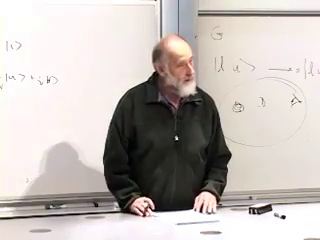
\includegraphics[width=0.66\textwidth]{lecture_07_figure_06.png}
\caption{Sự chuyển tiếp về mặt khái niệm từ một ket được chỉ rõ sang một mô tả theo tập hợp thống kê.}
\lectureframe{01:29:43}
\end{figure}

Nếu trạng thái \(|i\rangle\) được chuẩn bị với xác suất \(\rho_i\), thì toán tử mật độ là
\begin{equation}
\rho=\sum_i\rho_i|i\rangle\langle i|.
\end{equation}
Trong cơ sở chuẩn bị,
\begin{equation}
\rho=
\begin{pmatrix}
\rho_1&0&0&\cdots\\
0&\rho_2&0&\cdots\\
0&0&\rho_3&\cdots\\
\vdots&\vdots&\vdots&\ddots
\end{pmatrix}.
\end{equation}

\begin{figure}[htbp]
\centering
\includegraphics[width=0.68\textwidth]{lecture_07_figure_09.png}
\caption{Ma trận mật độ đường chéo và điều kiện chuẩn hóa của nó.}
\lectureframe{01:32:12}
\end{figure}

Các trị riêng của nó là thực và không âm, và điều kiện chuẩn hóa của các xác suất trở thành
\begin{equation}
\operatorname{Tr}\rho=\sum_i\rho_i=1.
\end{equation}

Cho \(F\) là một đại lượng quan sát Hermite. Giá trị kỳ vọng của tập hợp thống kê là
\begin{equation}
\langle F\rangle=\operatorname{Tr}(F\rho).
\end{equation}

\begin{figure}[htbp]
\centering
\includegraphics[width=0.68\textwidth]{lecture_07_figure_10.png}
\caption{Giá trị kỳ vọng dưới dạng vết \(\langle F\rangle=\operatorname{Tr}(F\rho)\).}
\lectureframe{01:35:05}
\end{figure}

Để thu lại trung bình có trọng số thông thường, hãy tính vết trong cơ sở mà \(\rho\) ở dạng đường chéo và chèn phân giải đơn vị:
\begin{align}
\operatorname{Tr}(F\rho)
&=\sum_i\langle i|F\rho|i\rangle\\
&=\sum_{i,j}\langle i|F|j\rangle
               \langle j|\rho|i\rangle\\
&=\sum_i\rho_i\langle i|F|i\rangle.
\end{align}
Vì vậy, mỗi giá trị kỳ vọng của trạng thái thuần được gán trọng số bằng xác suất mà trạng thái tương ứng đã được chuẩn bị.

Phép lấy vết có tính chất chu kỳ
\begin{equation}
\operatorname{Tr}(AB)=\operatorname{Tr}(BA),
\end{equation}
ngay cả khi \(A\) và \(B\) không giao hoán. Do đó \(\operatorname{Tr}(F\rho)=\operatorname{Tr}(\rho F)\).

\section{Entropy lượng tử và phần đền đáp đến sau}

Entropy của một ma trận mật độ là
\begin{equation}
S(\rho)=-\operatorname{Tr}(\rho\log\rho).
\end{equation}
Đối với một toán tử Hermite dương, các hàm như \(\log\rho\) được xác định thông qua các trị riêng của nó. Nếu
\begin{equation}
\rho=\sum_i\rho_i|i\rangle\langle i|,
\end{equation}
thì
\begin{equation}
\log\rho=\sum_{\rho_i>0}(\log\rho_i)|i\rangle\langle i|,
\end{equation}
và do đó
\begin{equation}
S(\rho)=-\sum_i\rho_i\log\rho_i.
\end{equation}

\begin{figure}[htbp]
\centering
\includegraphics[width=0.68\textwidth]{lecture_07_figure_11.png}
\caption{Công thức entropy cổ điển được viết lại dưới dạng \(S=-\operatorname{Tr}(\rho\log\rho)\).}
\lectureframe{01:41:25}
\end{figure}

Một trạng thái thuần đã biết có toán tử mật độ
\begin{equation}
\rho_\psi=|\psi\rangle\langle\psi|,
\end{equation}
với các trị riêng \(1,0,\ldots\), nên \(S(\rho_\psi)=0\). Điều này không có nghĩa là mọi phép đo trên \(|\psi\rangle\) đều có một kết quả chắc chắn. Nó có nghĩa là không còn sự thiếu thông tin thống kê bổ sung nào về trạng thái đã được chuẩn bị. Ở cực đối diện,
\begin{equation}
\rho=\frac{I}{d}
\qquad\Longrightarrow\qquad
S(\rho)=\log d,
\end{equation}
trong đó \(d=\dim\mathcal H\). Trạng thái trộn cực đại gán trọng số bằng nhau cho mọi hướng trực giao.

Mối liên hệ với rối lượng tử nay đã ở rất gần, nhưng vẫn chưa được triển khai. Giả sử một hệ hợp thành \(AB\) ở trong một trạng thái chung và mọi thí nghiệm đều chỉ giới hạn ở \(A\). Phải có một đối tượng tái tạo được mọi giá trị kỳ vọng có thể thu được trên \(A\) khi \(B\) bị bỏ qua. Đối tượng đó là một ma trận mật độ của \(A\). Nếu trạng thái chung có dạng tích, ma trận mật độ của \(A\) là thuần và có entropy bằng không. Nếu \(A\) và \(B\) ở trạng thái rối, ma trận mật độ của \(A\) nói chung là trộn và có entropy khác không. Việc xây dựng ma trận mật độ rút gọn đó và tính entropy của nó là nhiệm vụ được dành cho bài giảng tiếp theo.
